\def\QRCODE{TB_IPR_TUT.IMG.hough_matlabqrcode.png}
\def\QRPAGE{http://www.iptutorials.science/tree/master/TB_IPR/TUT.IMG.hough/matlab}
\mcorrectionsection{Matlab correction}

\subsection{Contour detection}


The first step is to perform contours detections. A classical method is employed here (see Fig.\ref{fig:tutorial:hough:matlab:canny}, Canny edge detection). The important thing is to start by a binary image (binary set of points).
\begin{matlab}
% Load an image
I  = double(imread('TestPR46.png'));
I = I(:,:,2); % keep grayscale image

%% performs contour detection
BW = edge(I,'canny');
\end{matlab}

\begin{figure}[htbp]
 \centering
 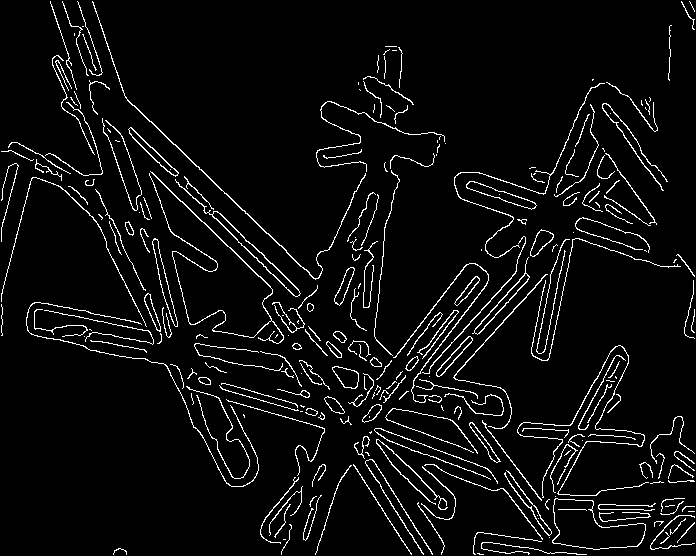
\includegraphics[width=6cm]{canny.png}
 \caption{Canny edge detection.}
 \label{fig:tutorial:hough:matlab:canny}
\end{figure}

\subsection{Hough transform}
This code does not make use of the \matlabregistered{} function dedicated to line detection.The result is presented in Fig.\iflabelexists{fig:tutorial:hough:results}{\ref{fig:tutorial:hough:results}.}{\ref{fig:tutorial:hough:matlab:result}.
	\begin{figure}[htbp]
	 \centering
	 
\includegraphics[width=8cm]{hough.png}
	 \caption{Hough transform.}
	 \label{fig:tutorial:hough:matlab:result}
	\end{figure}
}%

First, you can initialize the values. The size of the image is used to determine the maximal $\rho$ value.

\begin{matlab}
%% Hough transform
angular_sampling = 0.002; % angles in radians                                             
[x, y] = size(BW);

rho_max = norm([x y]);                                                
rho = -rho_max:1:rho_max;
theta = 0:angular_sampling:pi;
H = zeros(length(rho), length(theta));
\end{matlab}

Then, you loop over all the pixels $(i,j)$: in case of a True pixel (\minline{BW(i,j)==1}, you transform it into a sinusoid function, and increase the rounded values in the H matrix for all discrete values of $\theta$.

\begin{matlab}
% performs Hough transform
for i = 1:x
    for j = 1:y
        if BW(i, j)
            for theta_index = 1:length(theta)
                th = theta(theta_index);
                r  = i * cos(th) + j * sin(th);
                rho_index = round(r + length(rho)/2);                      
                H(rho_index, theta_index) = H(rho_index, theta_index) + 1;
            end
        end
    end
end
\end{matlab}


\subsection{Maxima detection}
\subsubsection{Basic maxima detection}
This version of maxima detection is very simple. However, it does not handle the neighborhood (it has the drawbacks of a basic threshold). One could look at h-maxima operators in order to get blobs instead of points. The threshold value can be tuned to find a given number of lines.

\begin{matlab}
%% maxima detection
difference = 50;
M = max(H(:));
maxima = H>(M-difference);

% find the peaks
[indices_rho_peaks, indices_theta_peaks] = find(maxima);
\end{matlab}

\subsubsection{Enhanced maxima detection}
The \matlabregistered{} version of the maxima detection gives cleaner maxima. Each peak, described by a coordinate $\rho, \theta$, corresponds to a line in the original image.
\begin{matlab}
peaks = houghpeaks(H, 5);
indices_rho_peaks   = peaks(:,1);
indices_theta_peaks = peaks(:,2);
\end{matlab}
The following code displays the results in the Hough space.
\begin{matlab}
rho_peaks   = rho(indices_rho_peaks);
theta_peaks = theta(indices_theta_peaks);

imshow(H,[]), hold on
title('Hough Transform');
xlabel('\theta (radians)');
ylabel('\rho (pixels)');
plot(indices_theta_peaks, indices_rho_peaks, 'r*');
\end{matlab}

\subsection{Lines retrieval}
From the coordinates $\rho, \theta$, it is easy to compute and display the different detected lines.
\begin{matlab}
%% Find hough lines
x= 1:size(I, 2);
figure, imshow(I,[]), hold on
for i=1:length(rho_peaks)
    y = (rho_peaks(i) - x* cos(theta_peaks(i)) )/ sin(theta_peaks(i));
    plot(y, x);
end
title('detected lines')
\end{matlab}
